\subsection{Episode 3: The Horse Whisperer}

\DndDropCapLine{T}he group begin in the bedroooms of the Tiki Tuks after the brutal, and controversial, murder of the "friendly" Tiki Tuk by Philo.\medskip

The goblins, unimpressed with this behaviour and sympathetic to the Tiki Tuks, head towards the treasure room.\medskip

A brief encounter in the water well room see Riphard unsuccessfully attempt to hold Pilch’s head underwater for more details on his violent nature, but Pilch is able to bat him away, swinging his head up in a glorious little mermaid inspired fashion. When asked why he killed the Tiki Tuk, Pilch looks genuinely conflicted.\medskip

Riphard wanders down an unknown corridor, much to Kolo's chagrin. Riphard explains that while Kolo just wants to find the treasure they know about, Riphard wants to find "the treasure that we don't know about”. Riphard is rewarded for his inquisitiveness by finding a stable full of boar and two more Tiki Tuks. Kolo is able to deescalate any possible fight using his language/diplomatic skills, thinking quickly on his feet about an alibi where he is actually visiting his uncle. The goblins laugh at the success of their favourite trick.\medskip

Riphard discovers another large corridor, this one lined with spiked walls and a mossy floor. Exme is able to discern that this used to be a booby-trapped room, however, it has long since fallen into disrepair. However, she does notice the strange fungus growing on the floor and harvests as much as she can along with her brother. Riphard is asked to help, but stubbornly refuses, not being one to do groundwork for such lowly creatures as goblins. Pilch is asked and curiously finds himself accepting the instructions.\medskip

The goblins head to the chief’s rooms. Exme discovers "nothing at all" in a room that she inspects, whilst Kolo recovers a strange, smooth, and intricately engraved stone under a pile of furs in the chief’s bedroom.\medskip

For some reason Pilch decides to argue that this might not be the fancy stone we have been sent here to find. Riphard queries just how many fancy looking stones Pilch thinks Tiki Tuks will have. Exme fumbles through her bag for a while, eventually pulling out a strange device which she passes over the stone. It delivers a small printed out piece of tape in Goblinese which she eyes before confirming that it is indeed the stone of Un’thala. Otoria is not surprised as she feels that most normal stones would not have received such careful treatment and preparation. The goblins inform the group that it is time to sleep, but the rest of the group resist the idea.\medskip

The group take some food from the stores, but are urged by Kolo to leave some for the Tiki Tuks. Kolo also leaves a message saying “nice to see you uncle”.\medskip

Pilch is racist.\medskip

The group travel for half a day, back towards Vathos Boundary, Exme noticeably struggling with her large and heavy bag. The group set up camp. Exme disappears for a short while and returns with herbs that she starts combining with the fungus in a small pestle and mortar. The entire group finds themselves falling asleep.\medskip

During their sleep they share a common dream in which Lazarus speaks to them and congratulates them on their progress so far. He lays out the next challenge, which is to head north to Hope’s Rest. He reveals Pilch perhaps has the closest connection to his kind. He instructs the group that they are to set up base in this liberal township, and will require money and transport to further their interests. The dream fades around the chuckles of Meredith.\medskip

The non-goblins in the group feel weary and drained.** Pilch** deduces that they may be suffering from Zukor’s Rot as a result of being shot with ancient darts in the Temple of Un'thala.\medskip

Exme hands Pilch a single packet of grey paste. She thanks him for his help in gathering the fungus, but berates him for his treatment of the murdered Tiki Tuk.\medskip

The group travel back to town and Otoria begins making inquiries concerning the exploding stable. Kolo and Exme mysteriously disappear. It is revealed that on top of this disaster, the town is now suffering from a spate of horse robberies, including those that led a caravan which is rumoured to be travelling to the north.\medskip

The group visit Black Smith the blacksmith where Kolo, mysteriously reappearing, requests new daggers. Exme, also mysteriously reappearing, attempts to hire the workshop to complete a project. Smith is initially dismissive, however his mind is changed rapidly when offered an ornate, solid gold necklace in return. The goblins begin their work, Exme concentrating hard on her work, and Kolo jumping maniacally on the bellows and hitting things with a hammer. The remaining members head to the titty bar.\medskip

Pilch tries some new, innovative ways of begging - he attempts hawks the Tiki masks as blood money, and gets a free drink from other alt-right extremists, but is told to sell the masks to the captain of the guard.\medskip

Riphard follows the blacksmith home and, once he has gone to bed, breaks into the man’s home and steals the necklace back. The rest of the group is unaware of this.\medskip

The group meet up in the morning and Riphard inquires where to fence sell "totally legitimate jewelry" in the town. He is directed to a jewelry shop where he is given a reduced price for the necklace. Shops have to make a profit, so that is completely normal practice and not a reflection on Riphard's bargaining skills.\medskip

The group head to the city guards offices to inquire about potential jobs and the stable mystery, that isn’t really that much of a mystery when you think about it because it was probably certainly a black powder gang or church related jobby.\medskip

They meet the half orc captain of the guard Urnok and his troll “friend?” Gumshoe. The group discusses local issues and learns more about how they may secure passage to the North.Kolo is a good detective gabrin. Riphard assures people he is a real pastor. Pilch sells 6 Tikki Tuk masks.\medskip

The following jobs are highlighted:\medskip

    Giant boar - Farmsteads in the North offering 50 gp to kill it.\\
    “Jennie’s girls” - Ex-whores who turned to crime after their profession was officially outlawed. Spread like herpes through the empire and can most likely be found to the north. Their leader is a woman called May or “some bitch called May”. The group is told t'arrest her, May.\\
    The SRA - Small Rights Activists. A collection of, mainly, gnomes and halflings who perform terrorists acts in their most-likely justified quest for improving the rights of smaller folk. Leader is Razzle Backshine, a gnome with a penchant for exploding things in people’s faces. Also spread out through empire.\\
    Diego Escabar and his Merry Men - A charming half elf who claims to steal from the rich and give to the poor, but doesn’t actually do the key last bit. Likely located in woodlands nearby. This is a local group.\medskip

Jobs are paid at a going rate of 5gp per severed left ear. Riphard wants to provide scalps, but is informed by Urnok that scalps are too easy to forge. Riphard accepts this explanation, explaining to the group that ears have a unique print, like fingers, which can be compared to the ear-print database the chief almost certainly keeps for this very purpose.\medskip

The gabrins try to turn Pilch in to the guards as Diego, but are unsuccessful. Riphard wonders whether Diego's men would live in a sort-of ghetto, a "robbing hood" if you will.\medskip

Pilch points out that it may be useful to try and recruit these groups, or at least align their interests with our own, and work together against the church.\medskip

Kolo asks Pilch if he has had sex. He replies that he totally has.\medskip

Riphard does not want to arouse suspicion and tries to persuade the group to let him visit the local pastor by himself. After some initial reservations the group allow him several minutes alone before they also insists on seeing the pastor themselves for no discernible reason or purpose.\medskip

Riphard's meeting with the pastor gets off to a tense start. “Are you here to help me?”. “Quite the opposite”. “You’re here to hinder me?”. Riphard questions the pastor on "the inquisition", but the pastor bats away his inquiries as mere tall tales. Riphard attempts to show the pastor proof of the inquisition by showing him the fatal wound he received that sent him to hell, but upon lifting his shirt finds his body shows no signs of trauma at all. The pastor tells Riphard he should ignore these scare stories. Riphard replies that in fact it is the pastor who should not ignore the warning signs. The rest of the group is unaware of this.\medskip

Riphard storms out and walks past the group without a word, looking very pissed off. The group take this as a sign to enter themselves.\medskip

Otoria and Pilch question the pastor, who has suddenly developed a tremendous stutter for some reason, and learn some things about how the Church operates, predominantly linked to their communication channels.\medskip

Riphard looks at boobs, too cheap pious to pay for a touch.\medskip

The group end up in the titty bar where Kolo is able to charm/seduce the busty barkeeper into revealing that she used to know May, back in the day. She reveals that May can be expected to be found to the east of the First River. The lady, flushed with lust towards the sweet-talking Kolo, retires to a back room to cool down. Kolo mysteriously disappears again.\medskip

The group spend a final night in the titty bar before setting off on their next adventure. As they sleep Lazarus visits them again to tell them that now they are in possession of the stone, some members may find themselves more attuned to any pre-existing magical conditions, but that this shouldn't affect their premiums.\medskip

\begin{center}
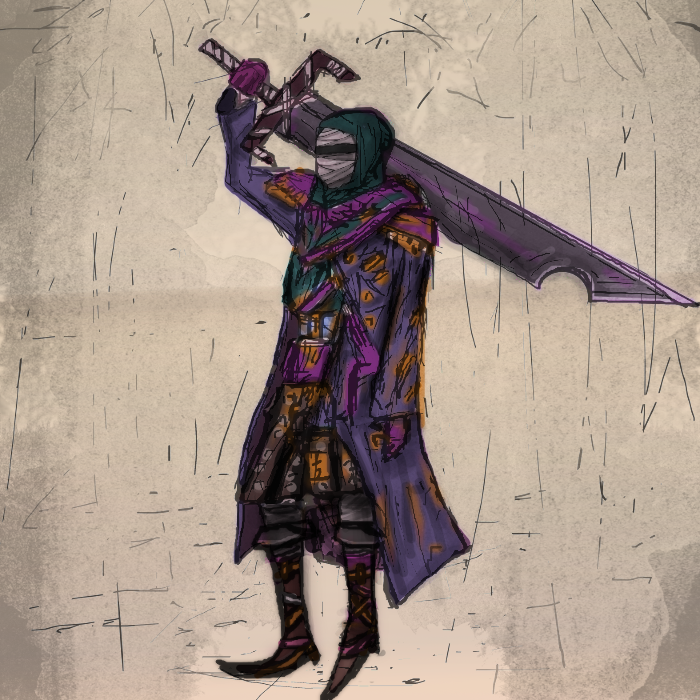
\includegraphics[width=80mm]{./content/img/otoria1.png}
\begin{figure}[h]
\end{figure}
\end{center}